\documentclass{article}
\usepackage{fullpage}
\usepackage{graphicx}

\newcommand{\sio}{{\tt spt-it-out}}

\title{\sio}
\author{Ethan Burns\\
{\tt burns.ethan at gmail.com}}
\date{\today}

\begin{document}
\maketitle

\section{Introduction}
\begin{center}
{\tt spt-it-out [<infile>]}
\end{center}

\sio\ is an interpreter for a small lisp-like language that can be
used to generate plots using the {\tt spt} library.  \sio\ can be used
as a batch program (when given an input file) or as a command-line
program (if no input file is specified).

\begin{figure}[t]
\begin{center}
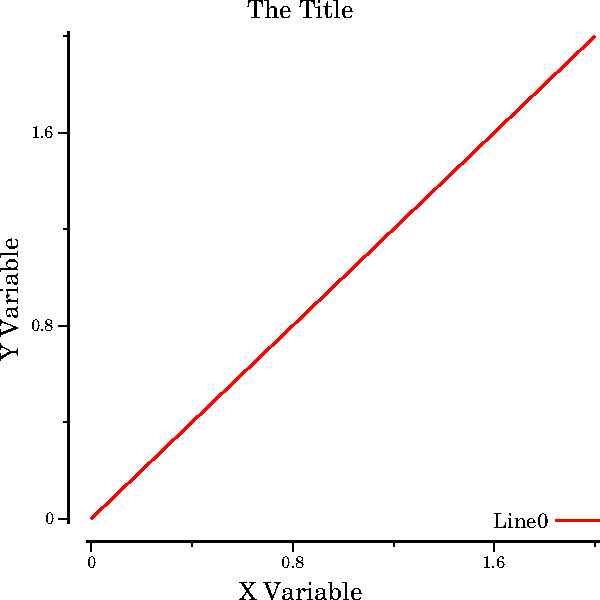
\includegraphics{simple_plot}
\caption{\label{fig:simp}A simple plot}
\end{center}
\end{figure}

\sio\ works by evaluating a plotting-expression.
Figure~\ref{fig:simp} shows the plot created from the simple
expression:

\begin{verbatim}
(output "simple_plot.pdf"
        (num-by-num-plot
         :title "The Title"
         :x-label "X Variable"
         :y-label "Y Variable"
         :legend (legend-location :lower-right)
         :dataset (line-dataset
                   :name "Line0"
                   :color (color :r 1.)
                   :points (points (0 0) (1 1) (2 2)))))
\end{verbatim}

The base expression is an {\tt output} expression.  The {\tt output}
expression takes two arguments: 1) The name of the output file as a
string and 2) A plot.  The second argument to this expression is a
numeric by numeric plot (one with both numeric x and y axes).  A
numeric by numeric plot is created with the {\tt num-by-num-plot}
function (described in more detail below).  The plot in this
expression has one dataset (the red line) which is specified by the
{\tt :dataset} option to the {\tt num-by-num-plot} function.  In this
case the dataset is a line dataset that is created with the {\tt
  line-dataset} function (again described further below).

As a convenience, \sio\ has a {\tt let} or {\tt let*} expression
similar to those found in lisp or scheme.  A {\tt let} expression
allows values to be bound to a variable names.  {\tt let*} is like let
except one binding can refer to the name bound by a previous binding
in the same binding list.  Using {\tt let*}, the previous expression
could be re-written:

\begin{verbatim}
(let* ((dataset0 (line-dataset
                  :name "Line0"
                  :color (color :r 1.)
                  :points (points (0 0) (1 1) (2 2))))
       (plot0 (num-by-num-plot
               :title "The Title"
               :x-label "X Variable"
               :y-label "Y Variable"
               :legend (legend-location :lower-right)
               :dataset dataset0)))
  (output "simple_plot.pdf" plot0))
\end{verbatim}

The following sections give detailed information on the functions
available in \sio.

\section{Getting Help}

The {\tt help} function can be used to get help on the available
functions in \sio.  Example:
\begin{verbatim}
> (help num-by-num-plot)
(num-by-num-plot [:title <string>] [:x-label <string>]
[:y-label <string>] [:width <length>] [:height <length>]
[:x-min <number>] [:x-max <number>] [:y-min <number>] [:y-max <number>]
[:dataset <num-by-num-dataset>]+)
Creates a plot with numeric x and y axes.
\end{verbatim}

\section{{\tt Output} and {\tt Display}}

\begin{description}

\item[{\tt (output <string> <plot>)}]
Output the given plot to the given
file.  The first argument is a file name string.  The extension given
in the file name dictates the output file format.  The format can be
any one supported by {\tt spt}: .pdf, .ps or .png.  The second
argument is a plot expression.

\item [{\tt (display <plot>)}] Displays the given plot using GTK.
\end{description}


\section{Numeric by Numeric Plots}

Numeric by numeric plots are standard plots with numeric x and y
axes.  They are created using the {\tt num-by-num-plot} function.  The
{\tt num-by-num-plot} function has the following options:

\begin{center}
\begin{tabular}{lll}
Option & Default & Notes \\
\hline
:title & & Plot title text\\
:x-label & & X label text\\
:y-label & & Y label text\\
:width & 4in & The width of the plot\\
:height & 4in & The height of the plot\\
:x-min & & The minimum x-axis value\\
:x-max & & The maximum x-axis value\\
:y-min & & The minimum y-axis value\\
:y-max & & The maximum y-axis value\\
:legend & :upper-right & The location of the legend \\
:dataset & & A dataset to add to the plot.  (See below for available
datasets).\\
\end{tabular}
\end{center}

The available legend locations are:

\begin{description}
\item[{\tt :upper-right}] Upper right corner of the plot.
\item[{\tt :upper-left}] Upper left corner of the plot.
\item[{\tt :lower-right}] Lower right corner of the plot.
\item[{\tt :lower-left}] Lower left corner of the plot.
\item[{\tt (legend-at <text-placement> <number> <number>)}] Puts the
  legend at a specified location.  <text-placement> is one of: {\tt
    :text-before} or {\tt :text-after} and the numbers are the x and y
  location of the legend.
\end{description}

\subsection{Numeric by Numeric Datasets}

The following are the available numeric by numeric datasets:

\subsubsection{\tt scatter-dataset}

Makes a dataset that displays a glyph at each of the given points.

\begin{center}
\begin{tabular}{lll}
Option & Default & Notes \\
\hline
:name & & The name, if not specified the dataset doesn't show in
the legend\\
:glyph & & ``circle'', ``ring'', ``cross'', ``plus'', ``square'',
``box'', ``triangle'' or string of len1\\
:color & & The color of the glyphs\\
:point-radius & 4pt & The radius of the glyphs\\
:points & & The data points\\
\end{tabular}
\end{center}

If {\tt :glyph} is not specified then the next glyph is used in a
default list of glyphs.

Note: if more than one {\tt :points} options are specified the
behavior is to concatenate the points into one single list of points.

\subsubsection{\tt bestfit-dataset}

Makes a dataset that displays a glyph at each of the given points with
a best linear fit line.  The options are the same as for {\tt
  scatter-dataset} except the following additional option is
available.

\begin{center}
\begin{tabular}{lll}
Option & Default & Notes \\
\hline
:dashes & & A list of lengths {\tt (<on> <off> ...)} that specify the
dash pattern of the line\\
\end{tabular}
\end{center}

If {\tt :dashes} is not specified then the next in a default list of
dash patterns is used.

\subsubsection{\tt bubble-dataset}

Creates a bubble plot.  This is like a scatter plot but the data is
specified in triples {\tt (<i> <j> <k>)} where the first and second
value are the x and y coordinates of the bubble and the third value is
used to specify the size of the bubble.  The options are the same as
for {\tt scatter-dataset} except instead of {\tt :point-radius} the
minimum and maximum radius are given and the data is given in triples
instead of points:

\begin{center}
\begin{tabular}{lll}
Option & Default & Notes \\
\hline
:min-radius & 10pt & The minimum radius of a bubble\\
:max-radius & 60pt & The maximum radius of a bubble\\
:triples & & The data\\
\end{tabular}
\end{center}

\subsubsection{\tt line-dataset}

A line dataset.  This draws a simple line.

\begin{center}
\begin{tabular}{lll}
Option & Default & Notes \\
\hline
:name & & The name, if not specified the dataset doesn't show in
the legend\\
:dashes & & A list of lengths {\tt (<on> <off> ...)} that specify the
dash pattern of the line\\
:color & & The color of the line\\
:line-width & 1pt & The width of the line\\
:points & & The data points\\
\end{tabular}
\end{center}

If {\tt :dashes} is not specified then the next in a default list of
dash patterns is used.

\subsubsection{\tt line-points-dataset}

A line with glyphs drawn at each point.  This dataset has the same
options as {\tt scatter-dataset} and {\tt line-dataset}.

\subsubsection{\tt line-errbar-dataset}

This dataset is given a set of lines.  The plot shows the interpolated
mean value line with error bars showing a 95\% confidence interval.

\begin{center}
\begin{tabular}{lll}
Option & Default & Notes \\
\hline
:name & & The name, if not specified the dataset doesn't show in
the legend\\
:dashes & & A list of lengths {\tt (<on> <off> ...)} that specify the
dash pattern of the line\\
:color & & The color of the line\\
:line-width & 1pt & The width of the line\\
:lines & & A list of point lists (lines).  Each set of points should
be sorted on x.\\
\end{tabular}
\end{center}

As an example, the following expression will create the plot shown in
Figure~\ref{fig:line_err}:

\begin{verbatim}
(let* ((line0 (points (0 0) (1 1) (2 2)))
       (line1 (points (0 -1) (1 0) (2 1)))
       (line2 (points (0 1) (1 2) (2 3)))
       (dataset0 (line-errbar-dataset
                  :name "Line with errar bars"
                  :lines (line0 line1 line2)))
       (plot0 (num-by-num-plot
               :legend (legend-location :lower-right)
               :dataset dataset0)))
  (output "line_err.pdf" plot0))
\end{verbatim}

\begin{figure}[t]
\begin{center}
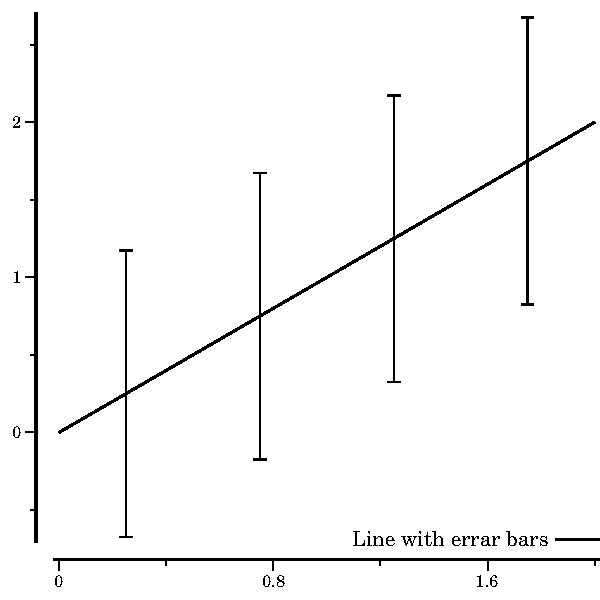
\includegraphics{line_err}
\caption{\label{fig:line_err}A mean-line with error bars plot.}
\end{center}
\end{figure}

\subsubsection{\tt histogram-dataset}

A histogram shows a distribution of values.

\begin{center}
\begin{tabular}{lll}
Option & Default & Notes \\
\hline
:name & & The name, if not specified the dataset doesn't show in
the legend\\
:dashes & & A list of lengths {\tt (<on> <off> ...)} that specify the
dash pattern of the line\\
:color & & The color of the line\\
:line-width & 1pt & The width of the line\\
:bin-width &  & The width each bin\\
:values & & A list of scalar values.\\
\end{tabular}
\end{center}

The default bin width creates 10 bars.  {\tt :line-width} and {\tt
  :dashes} control the look of the line forming the bars of the
histogram.

\subsubsection{\tt cdf-dataset}

A histogram shows a cumulative distribution of values.
The options are the same as for a histogram except that there is no
{\tt :bin-width} option.

\subsubsection{\tt num-by-num-composite}

New datasets can be created by putting other datasets together.  For
example, the following expression will create a step function shown in
Figure~\ref{fig:step} by compositing three line datasets:

\begin{verbatim}
(let* ((line0 (points (0 0) (1 0)))
       (line1 (points (1 1) (2 1)))
       (line2 (points (2 2) (3 2)))
       (line-ds0 (line-dataset :dashes () :points line0))
       (line-ds1 (line-dataset :dashes () :points line1))
       (line-ds2 (line-dataset :dashes () :points line2))
       (dataset0 (num-by-num-composite
                  :name "Step function"
                  :dataset line-ds0
                  :dataset line-ds1
                  :dataset line-ds2))
       (plot0 (num-by-num-plot
               :legend (legend-location :lower-right)
               :dataset dataset0)))
  (output "step_func.pdf" plot0))
\end{verbatim}

\begin{figure}[t]
\begin{center}
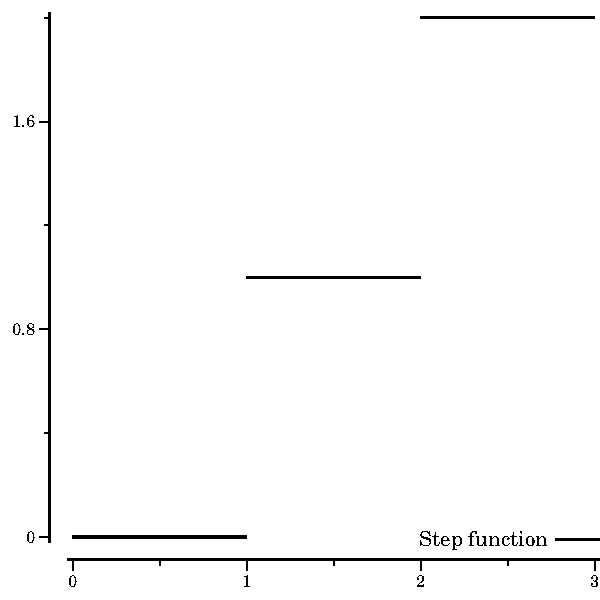
\includegraphics{step_func}
\caption{\label{fig:step}A simple step-function.}
\end{center}
\end{figure}

\section{Numeric by Nominal Plots}

Numeric by nominal plots are plots with an numeric y-axis but a
nominal x axis.  In this type if plot, each dataset is allocated a
fixed width of the x axis into which it will be displayed.

\end{document}
